\chapter{Gene Discovery through Plant Genome Environment Associations:
The Case for Enhanced Machine Learning Models of Soil Phosphorus Availability}
\label{chap-three}

\newrefsection

\section{Abstract}

\section{Background}

%% \caption[Evidence of highland selection in genes determining PC/LPC ratios]{\textbf{\textit{Evidence of highland selection in genes determining PC/LPC ratios.}}
%%  \textbf{(A)}
 
\begin{figure}[!ht]
\centering
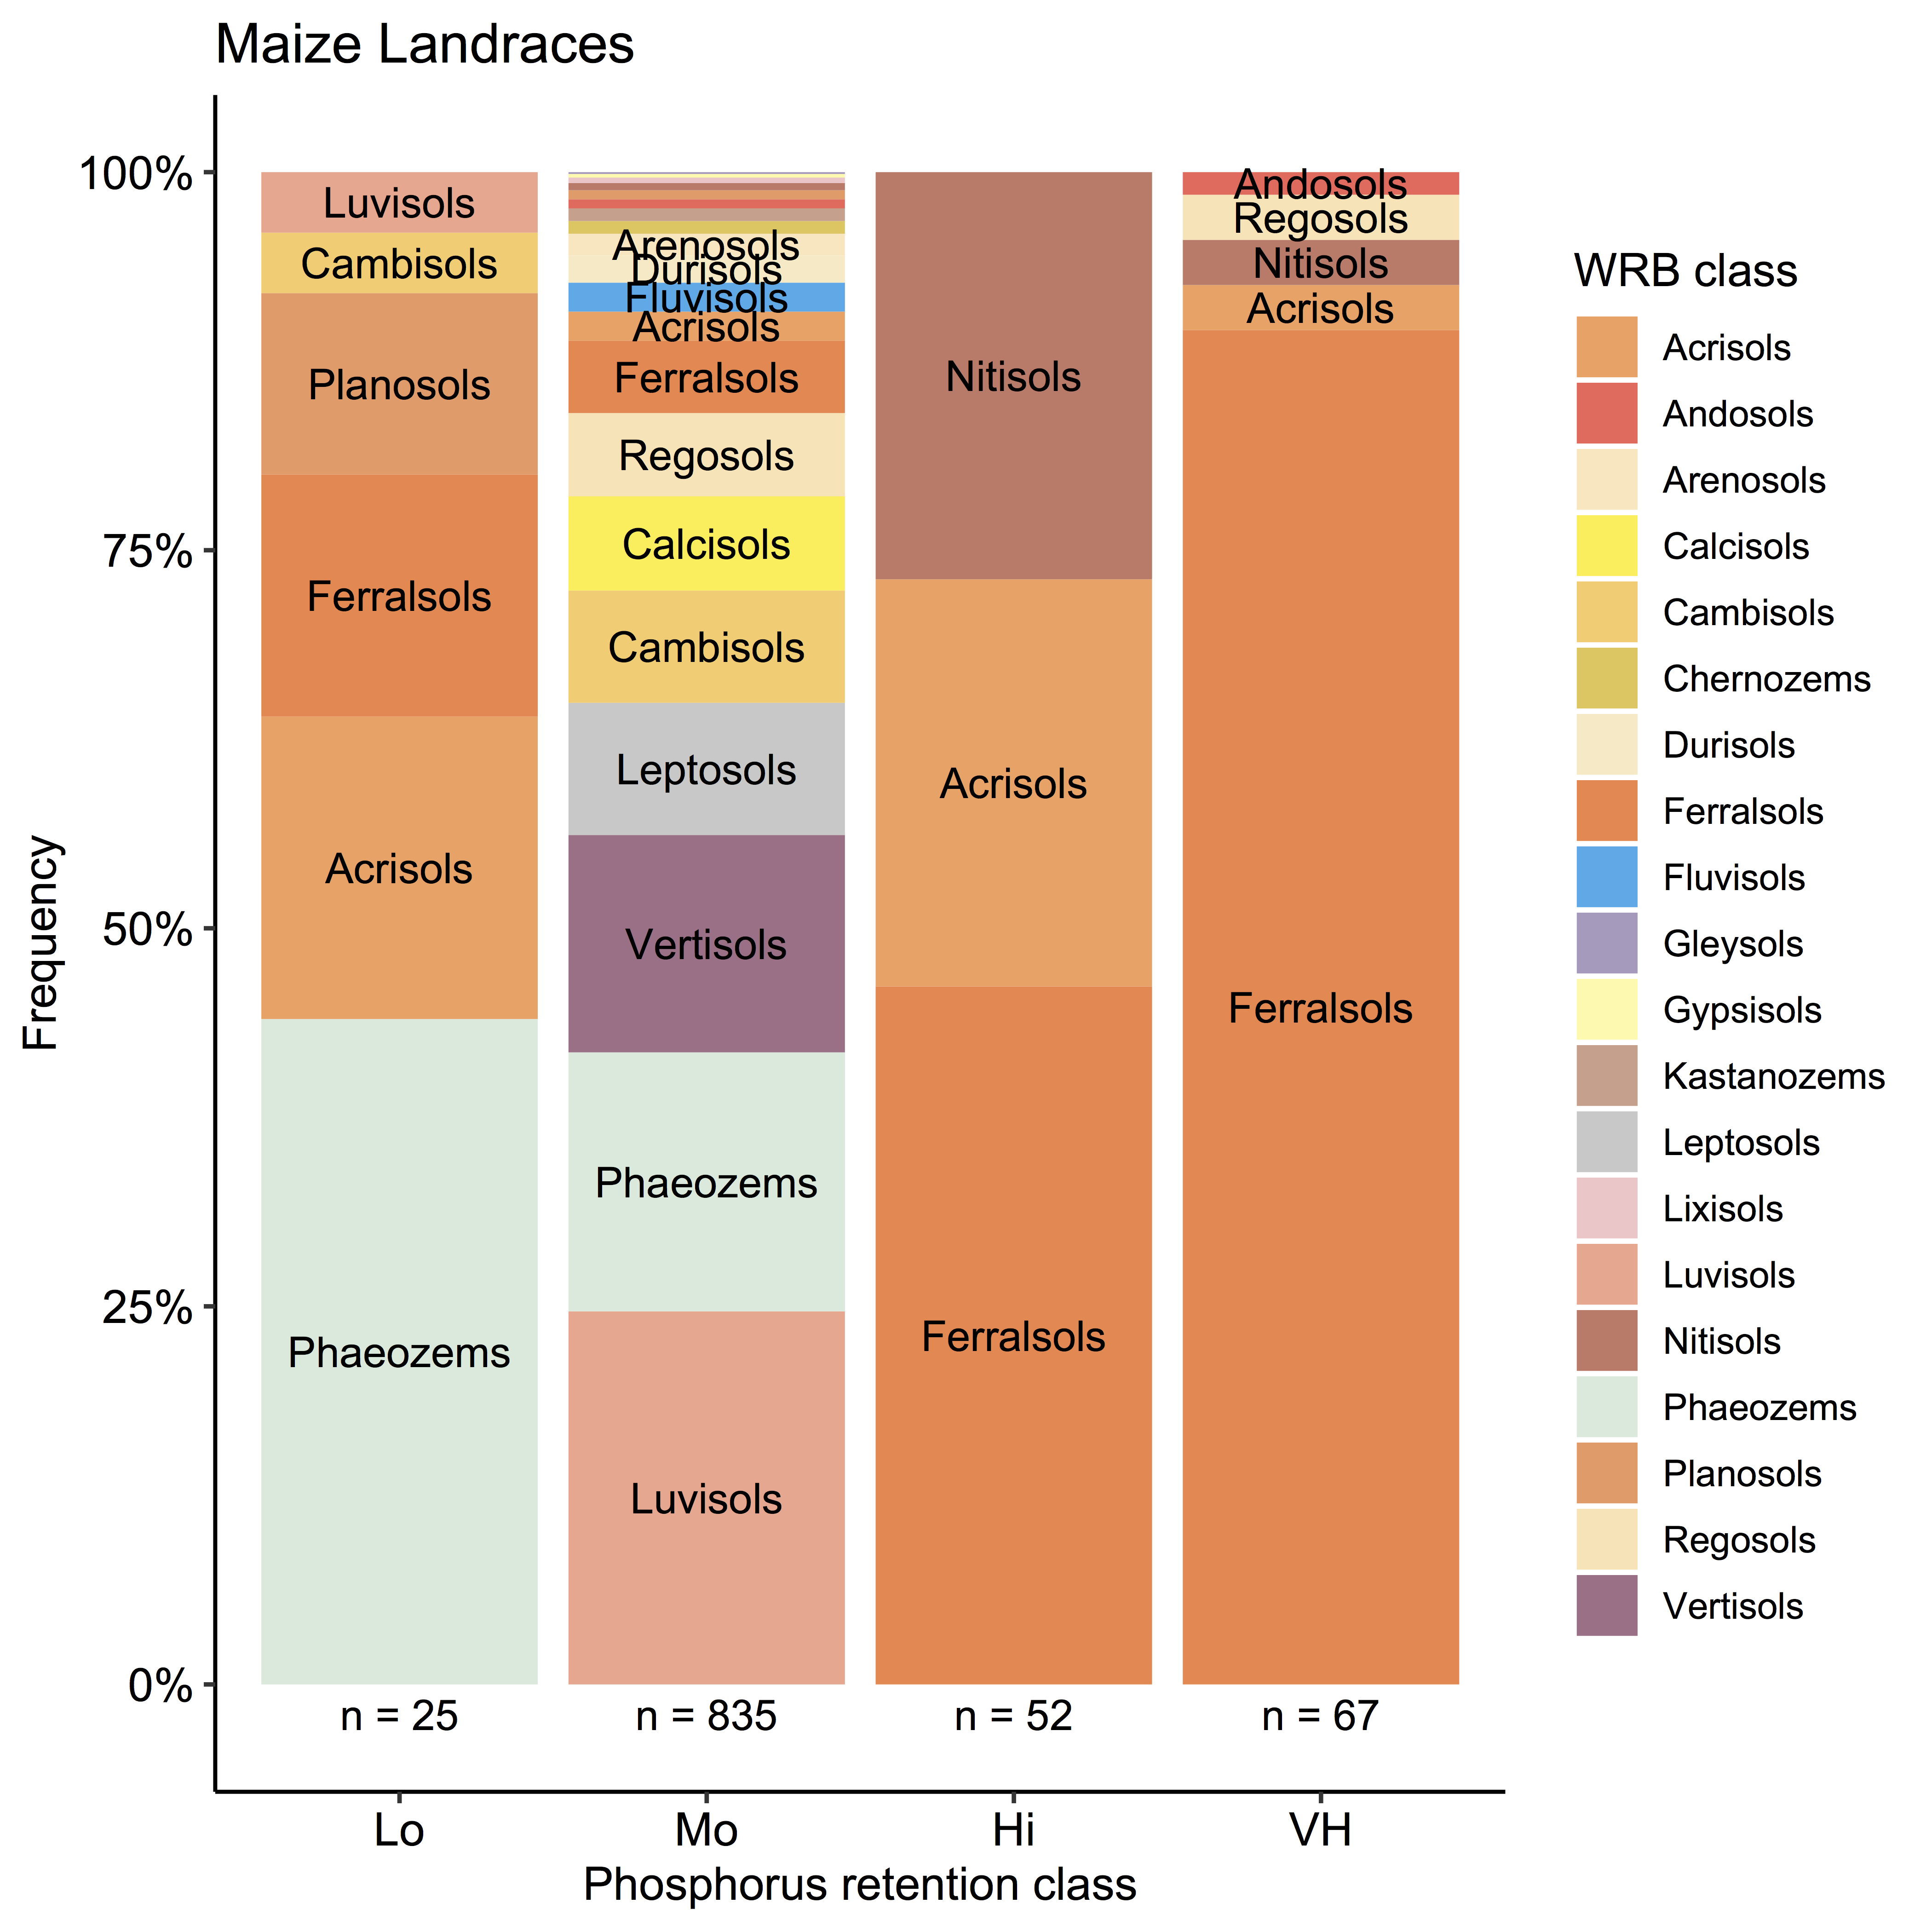
\includegraphics[width=\linewidth]{Chapter-2/figs/WRB_Pret.png}
\caption[Phosphorus Retention Potential For Maize Traditional Varieties in Latin America and the Caribbean]{\textbf{\textit{Phosphorus Retention Potential For Maize Traditional Varieties in Latin America and the Caribbean.}}
Based on \citep{batjes2011}.  Each soil unit corresponds to a mineral descriptor, e.g. Acrisol soil units can be gleyic, humic, orthic, or plinthic. Ferric acrisols have very low phosphorus solubility potential (first column), the other three acrisol units have low solubility (second column). The soil groups with predominantly High and Very High solubility are Ferralsols, Andosols, Acrisols, and Nitosols.}
\label{fig::WRB_Pret}
\end{figure}
\clearpage

\section{Methods}
\subsection*{Building and Validating a Model for Plant Available Phosphorus Distribution in Mexico}

To find associations between plant-available soil phosphorus and the genetic diversity of maize traditional varieties, I started by compiling public datasets on global phosphorus distribution. Because of it's high resolution and interepretability I intended to use the Olsen \citep{olsen1954} phosphorus predictions by \citep{mcdowell2023}, however this model shows no predictive value (Pearson correlation $r=0.076$) for the 500 samples coming from Latin America and the Caribbean present in that data set.

In addition to \citep{mcdowell2023}, I searched for other datasets and parameters that could be correlated to experimental measures of plant-available phosphorus in soils.
These included total phosphorus from \citep{hexianjin2022}, labile and total phosphorus from \citep{yang2013}, phosphorus by Bray, Olsen and Mehlich \citep{mehlich1984} methods, New Zealand phosphorus retention from \citep{shangguan2014} and NP limitation from \citep{du2020}.
However, I found no useful correlation (Pearson $r < 0.1$) between the \citep{mcdowell2023} experimental Olsen and Bray data and any of the reported predictions for those geolocalized soil profiles.

As the global databases had a very low predictive value for plant available soil phosphorus in Latin America, I narrowed the scope and focused to the Mexican territory and used the published data from the Instituto Nacional de Estadística y Geografía \citep{paz-pellat2018} from georeferenced soil profiles collected between 1969 to 2006.
This set contained topsoil phosphorus measurements as extractable phosphorus concentration in ppm [mg/kg] for 13092 gelolocalized soil profiles, divided into 8325 datapoints for  Olsen phosphorus (soils $\text{pH} > 7$) and 4767 datapoints for Bray phosphorus  (soils with $\text{pH} \leq 7$) for Mexico. 

For investigating the phosphorus distribution among different soil types according to WRB taxonomy \citep{wrb2014},  I used the field determinations of WRB soil group for the INEGI Serie II data \citep{inegi2013} and corresponding interpretation \citep{inegi2011,inegi2009} that matched both in  geolocation to (within a 150m) and profile identifier. 

Then I followed the random forest based methodology for soil predictive mapping developed by \citep{hexianjin2022} for its demonstrated prediction value for total phosophorus, interpretability, and computational time savings in comparison with the more onerous 150 input variable models of \citep{hengl2019} or \citep{mcdowell2023}. 
Here I used the maps for 16 predictors of available phosphorus and improving data clean up and resolution where possible.
The predictors were as follows: Mean Annual Temperature and Mean Annual Precipitation from BioClim 2.0 at 10 km resultion \citep{fick2017}; WRB soil groups at 10 km and pH, soil organic carbon, bulk density at 250 m resolution, from SoilGrids 250 \citep{hengl2019,hengl2017,wrb2022,scheffe2015}, USDA taxonomy order from OpenLandMap at 250 m, biomes fom Resolve Ecoregions \citep{dinerstein2017} at 10 km, Mean Annual Net Primary Production from MODIS \citep{running2015a}, elevation 15 m from INEGI CEM 3.0 \citep{inegi2019}, slope 1 km from EarthEnv \citep{amatulli2018}, soil depth at 10 km from Land-Atmosphere Interaction Research Group \citep{shangguan2017}, and lithology from GLiM rasterized at 10 km resolution\citep{hartmann2012}(details on Suplementary file S1).
All coordinates were matched to WGS84 latitude longitude for extraction of values from each raster using the custom R scripts.
I used this dataset for point predictions and so I refer to this data set as the POINTDATA.

I ran 15 simple random forest model with these 16 predictors and a single response variable using the R library `randomForest` \citep{liaw2002}. 
Either I used as output variable just the Bray measurements, the Olsen measurements, or a synthetic variable I called PHOS that consisted in the union of those two sets of observations, i.e. the PHOS parameter is a measure of phosphorus availability in the soil that corresponds to Bray I extractable phosphorus if the soil $\text{pH} \leq 7$ and to the Olsen extractable phosphorus if the soil $\text{pH} > 7$. 
I followed the code used by \citep{hexianjin2022}  with 3 random variables selected at each decision node, 500 trees per model, $70\%$ training, $30\%$ testing data a 5 fold cross validation at each step.
The predictive value of the model is measured as the Pearson correlation between the observed experimental values of available phosphorus concentration and the prediction from the random forest in the test data. 
The cross validation was used to measure the contribution of each predictor to the model by removing it from the model and measuring the resulting change in mean standard error of the prediction as a percentage. 
Additionally I ran an ensemble model based on the 15 outputs of the simple random forest model to see if it would increase predictive values in the test data.
Although I increased the correlation between observations an predictions using the ensemble model, I did not observed a improvement in the test predictions worthy both the more complicated model.

The POINTDATA needed additional matching in resolution and projection for making a raster prediction at 10 km resolution. So in  I used  \href{https://github.com/sawers-rellan-labs/grassGEA}{a series of custom $`R`$ language scripts} based on the `raster`, `gdal`, `sp` and `stars` libraries for obtaining 15 10km ($0.8883 \times 0.9993$ decimal degrees) latitude longitude WGS84 rasters. This dataset will be referred as MAPDATA.

\subsection*{Gene Environment Association}

\section{Results}

\begin{figure}[!ht]
\centering
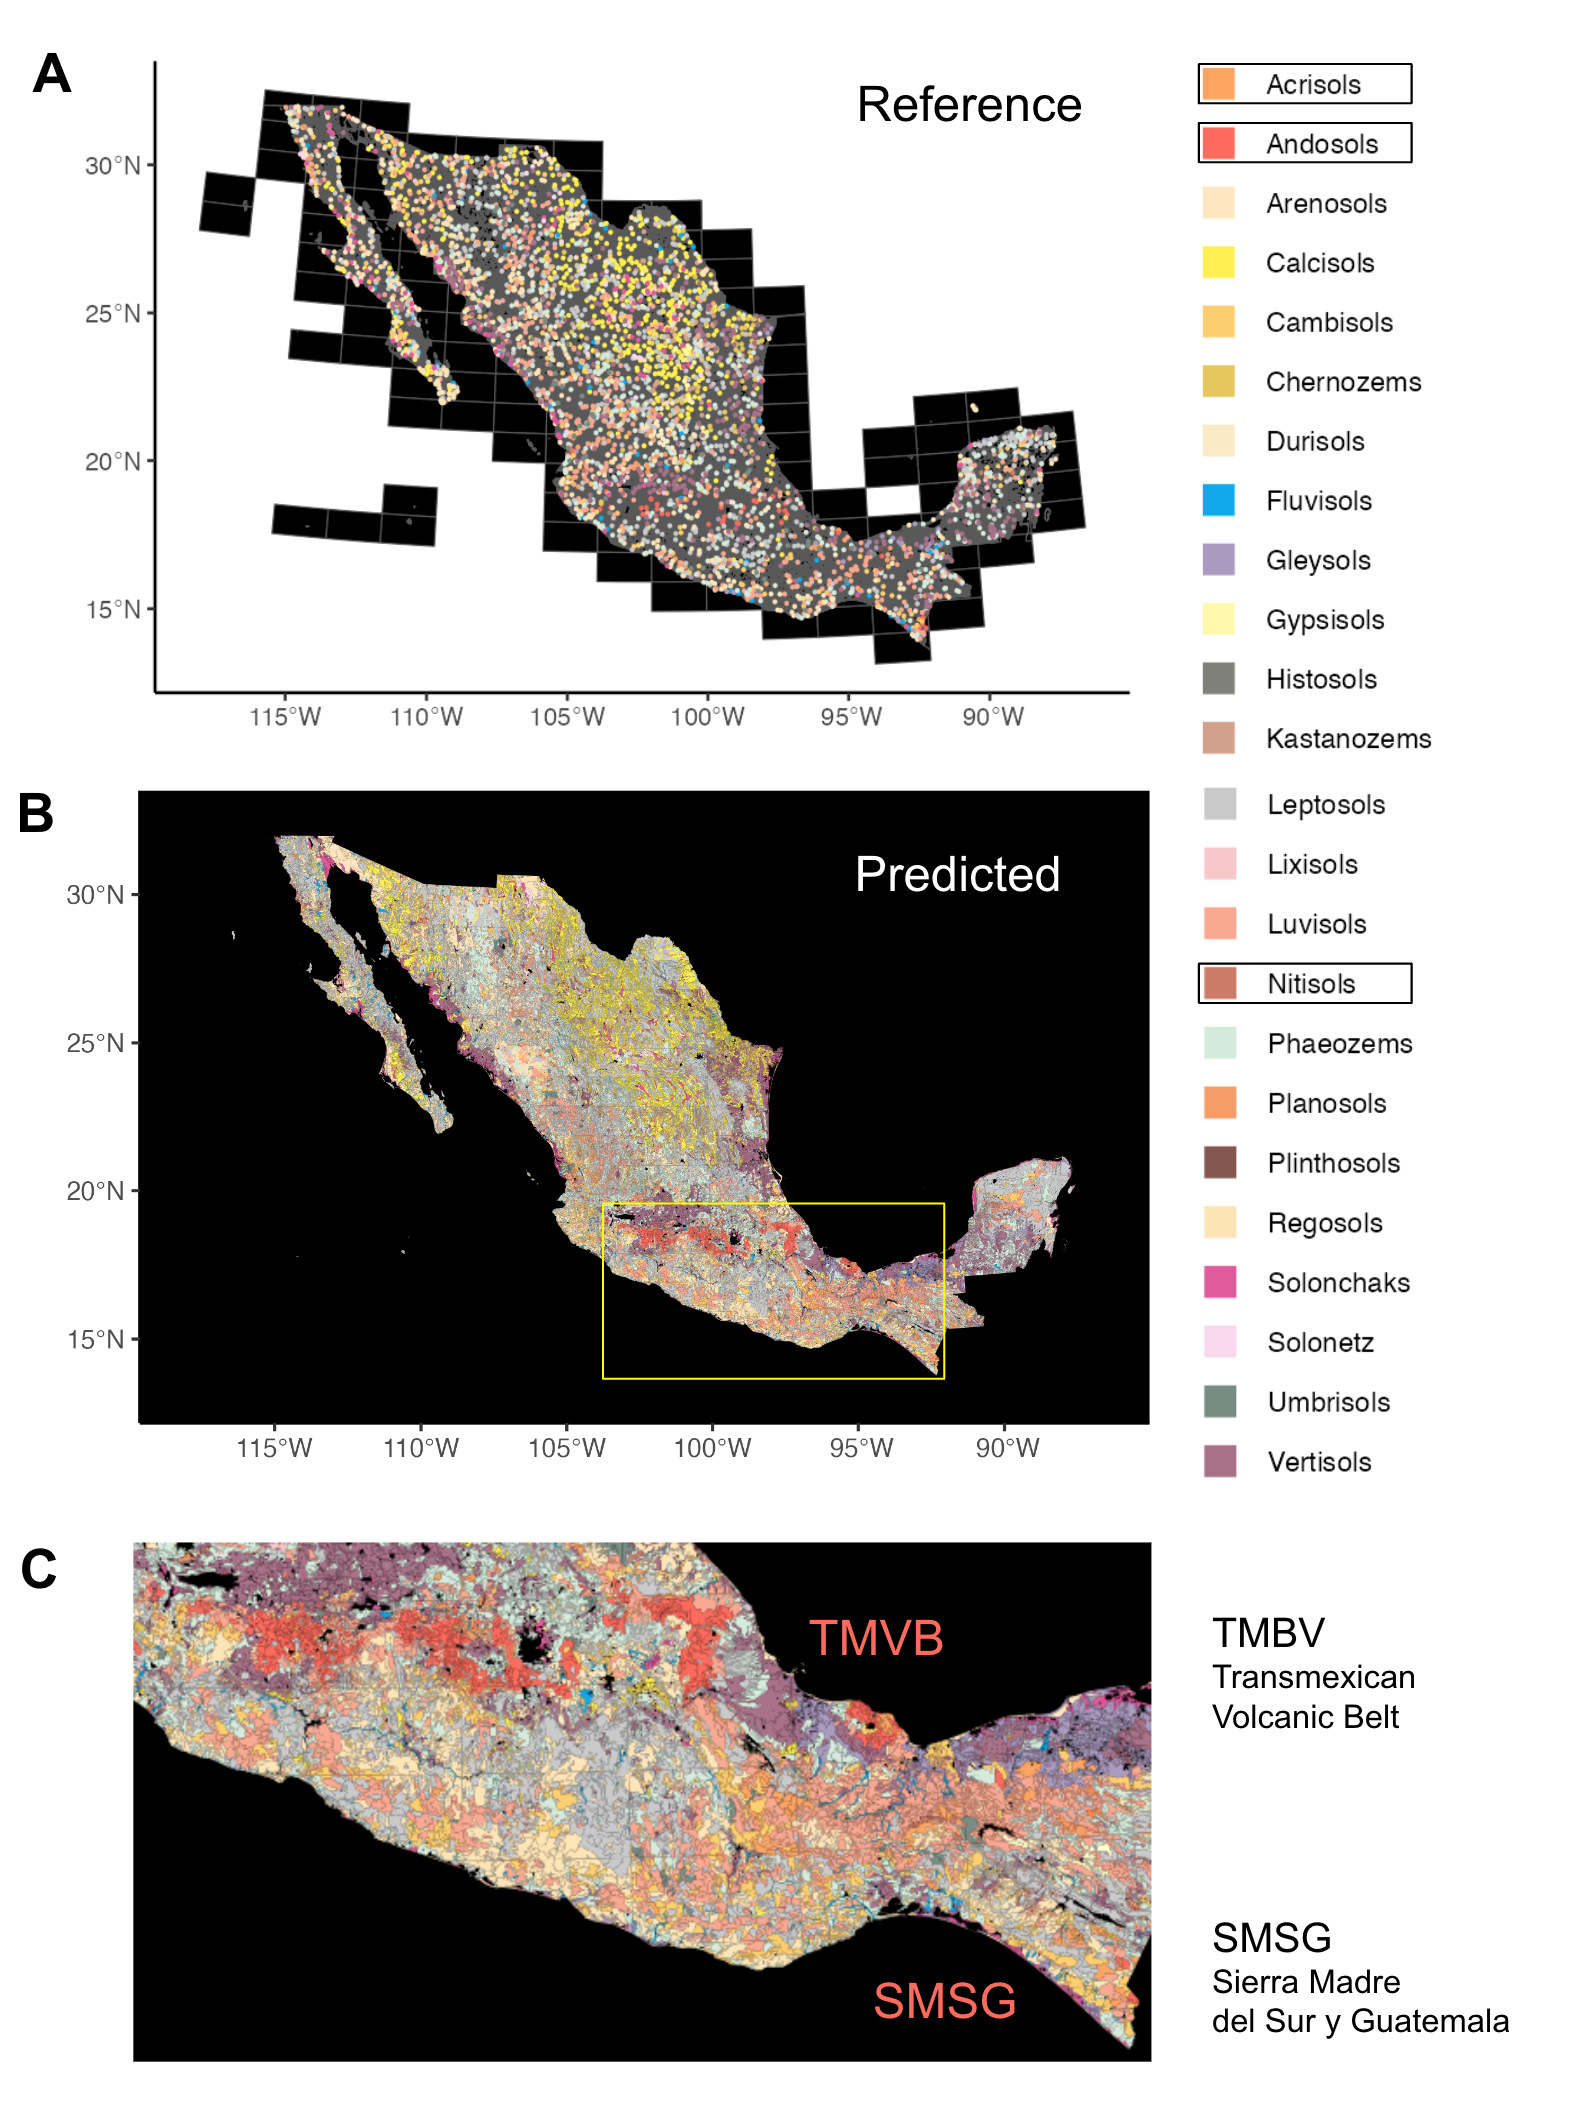
\includegraphics[width=0.9\linewidth]{Chapter-2/figs/WRB_inegi2013map.png}
\caption[WRB Soil Group Classification for Mexican soils according to INEGII]{\textit{\textbf{WRB Soil Group Classification for Mexican soils according to INEGI.}} \\\hspace{\textwidth}
\textbf{(A)} Reference soil profiles (n=4000) \citep{inegi2013}.
\textbf{(B)} 1:250000 map prediction for the dominant WRB soil group \citep{inegi2015} \textbf{(C)} Andosols predominate in the Transmexican Volcanic Belt at high altitudes and are frequent in the Sierra Nevada de Chiapas y Guatemala, collection areas for the Andosol Introgression Resource population (chapter 4)}
\label{fig::WRB_inegi2013map}
\end{figure}
\clearpage




\begin{figure}[!ht]
\centering
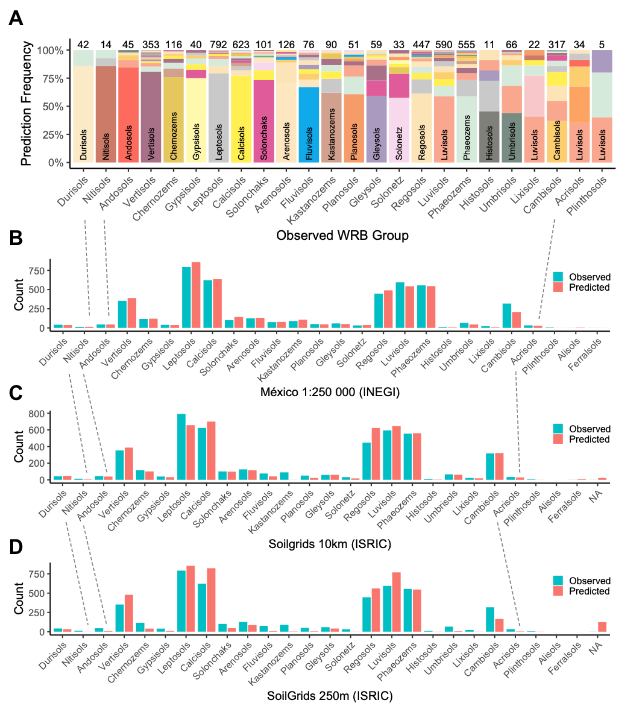
\includegraphics[width=\linewidth]{Chapter-2/figs/WRB_inegi_soilgrids}
\caption[Comparison between INEGI and SoilGrids WRB soil Classification Maps]{\textit{\textbf{Comparison between INEGI and SoilGrids WRB soil Classification maps.}} \\\hspace{\textwidth}
\textbf{(A)} INEGI 1:250000 map dominant soil prediction sorted by AUROC, total count above the bar. From Histosols to the right misclassifications are more common than correct classifications. For Lixisisols, Cambisols, Acrisols and Plinthosols the most frequent prediction does not match the observed soil group.
\textbf{(B)}  INEGI 1:250000 map dominant soil prediction in absolute frequency scale (count), same as the number of top of A bars.
\textbf{(C)} Soilgrids 10 km WRB dominant soil prediction. Downscaled resolution from 250 m.
\textbf{(D)} Soilgrids 250 WRB dominant soil prediction, it  has more missing data and underpredicts Andosols}
\label{fig::WRB_inegi2013map}
\end{figure}
\clearpage


\begin{figure}[!ht]
\centering
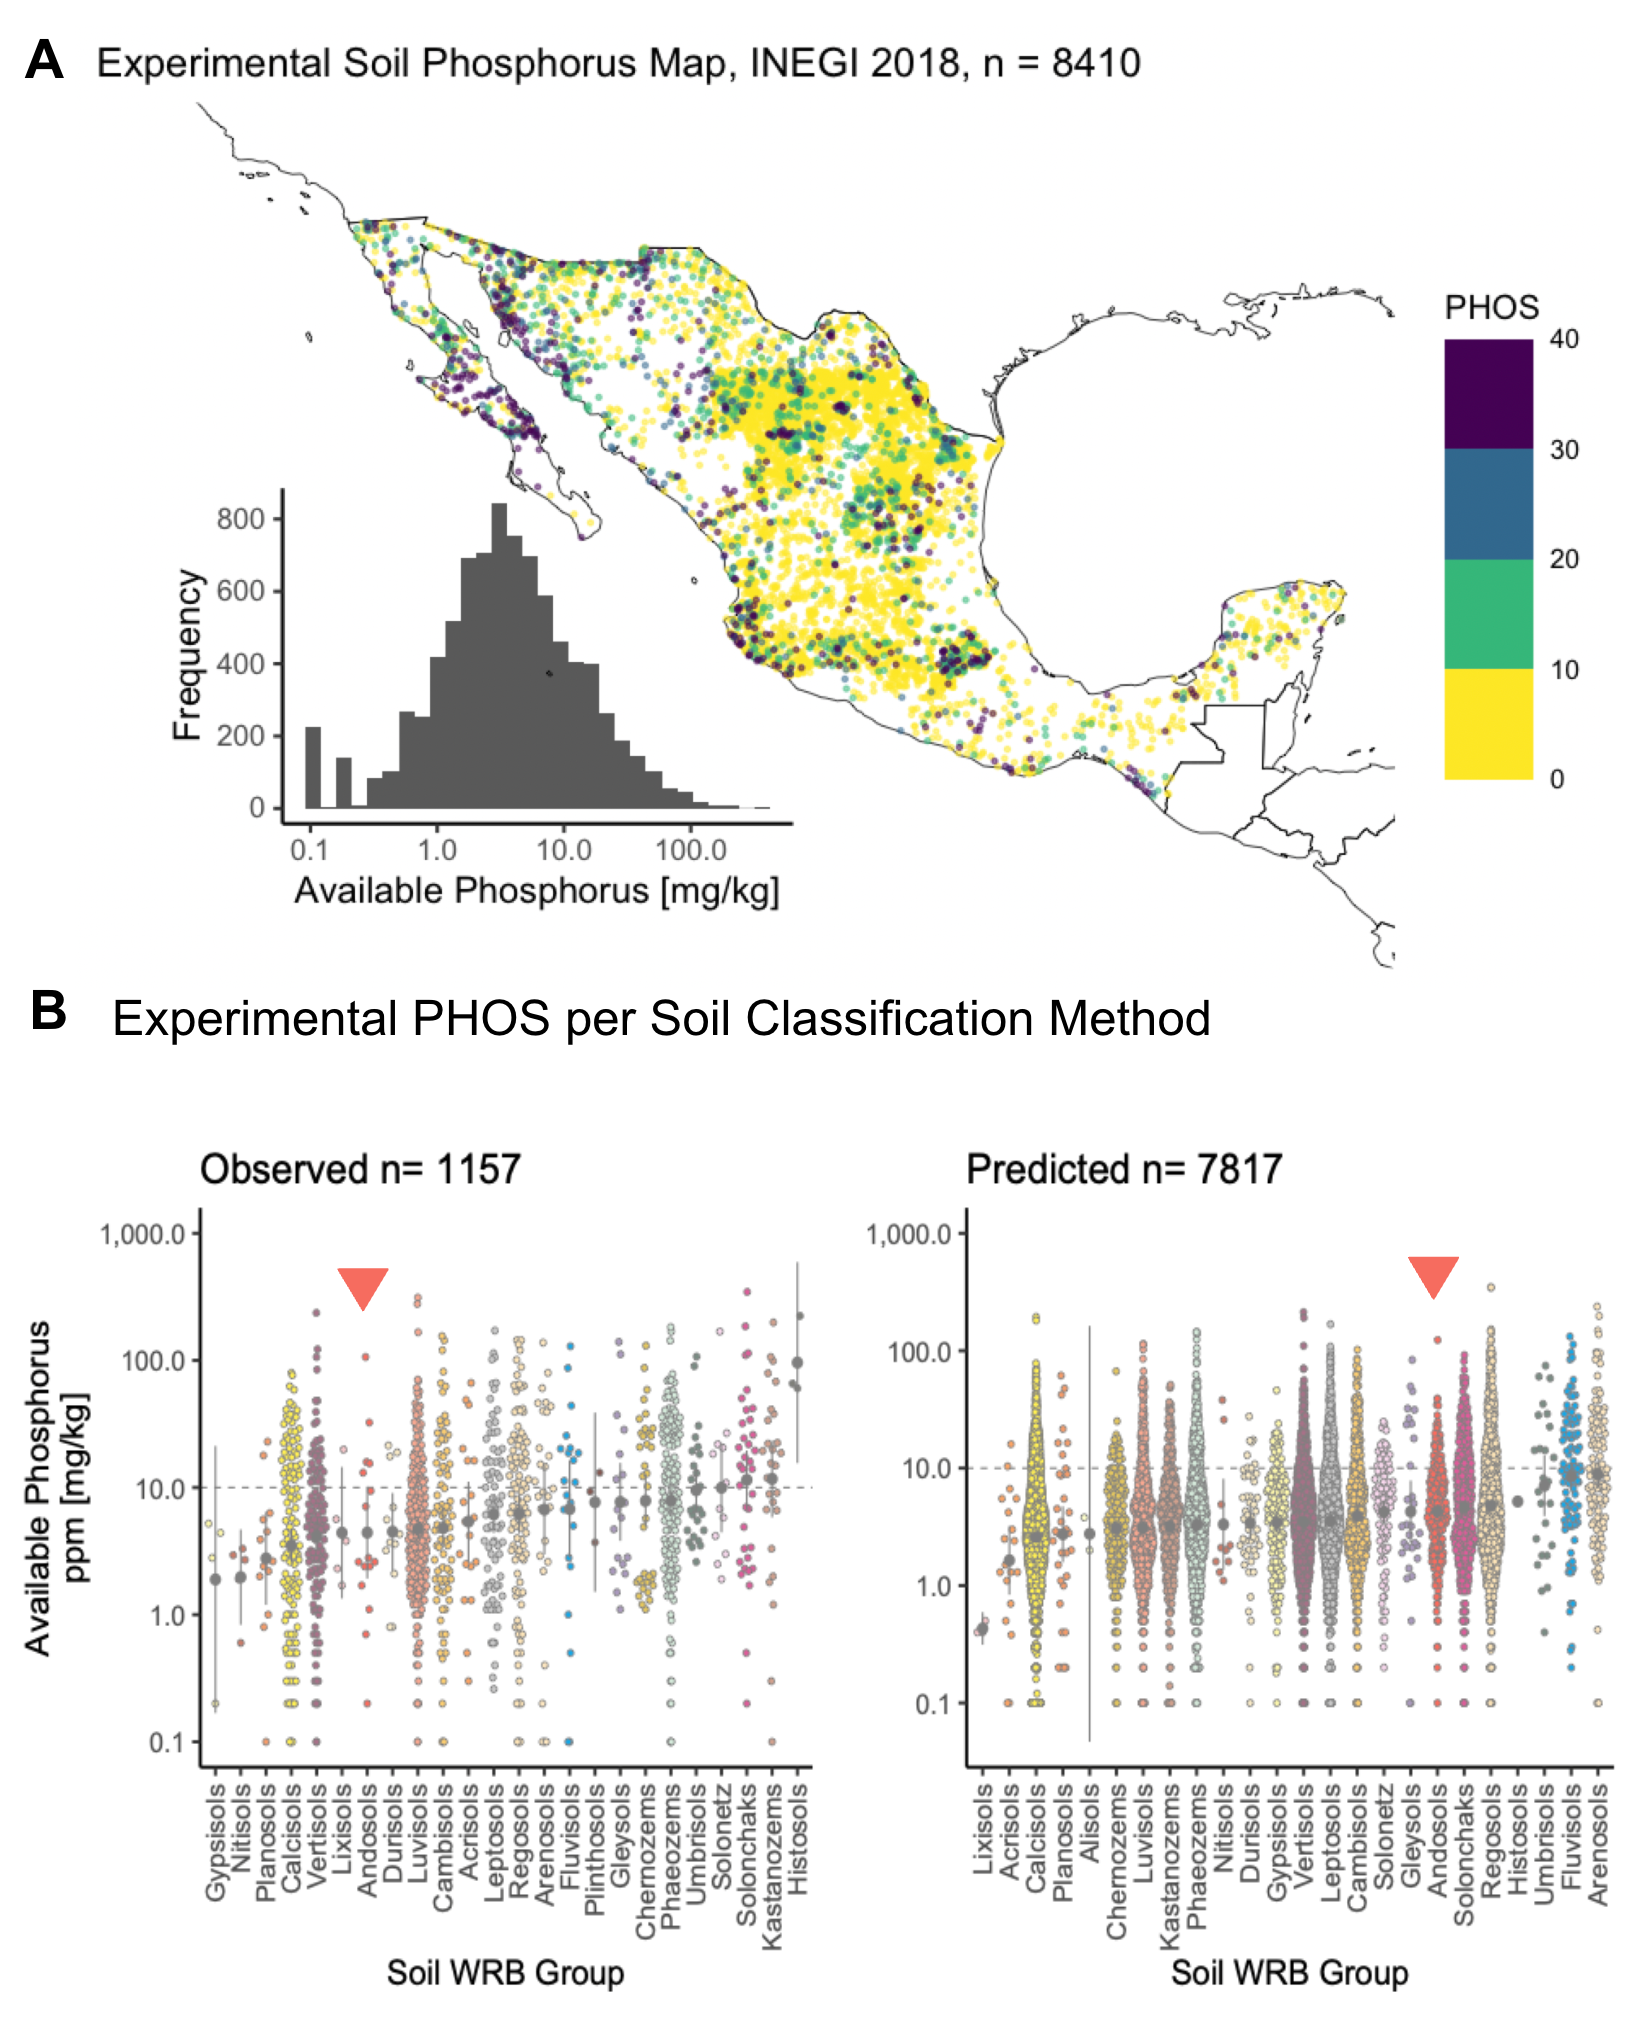
\includegraphics[width=0.65\paperwidth]{Chapter-2/figs/obeserved_PHOS.png}
\caption[Experimental values for topsoil plant available phosphorus (PHOS) in Mexico]{\textit{\textbf{Experimental values for topsoil plant available phosphorus (PHOS) in Mexico.}} \\\hspace{\textwidth} 
\textbf{(A)} Geographical distribution of sampled soil profiles. For acid and neutral soils ($\text{pH} \leq 7$) the reported PHOS value corresponds to Bray I phosphorus. For basic soils, Olsen phosphorus is reported as PHOS \citep{paz-pellat2018}.
\textbf{(B)} Available phosphorus per WRB soil group determination method, \textit{left:} observed WRB determination in the field for INEGI reference profiles, \textit{right:} assignation of dominant soil in the corresponding map unit (polygon) in \citep{inegi2013}. Downward triangle points to Andosol group soils}
\label{fig::WRB_inegi2013map}
\end{figure}
\clearpage

\begin{figure}[!ht]
\centering
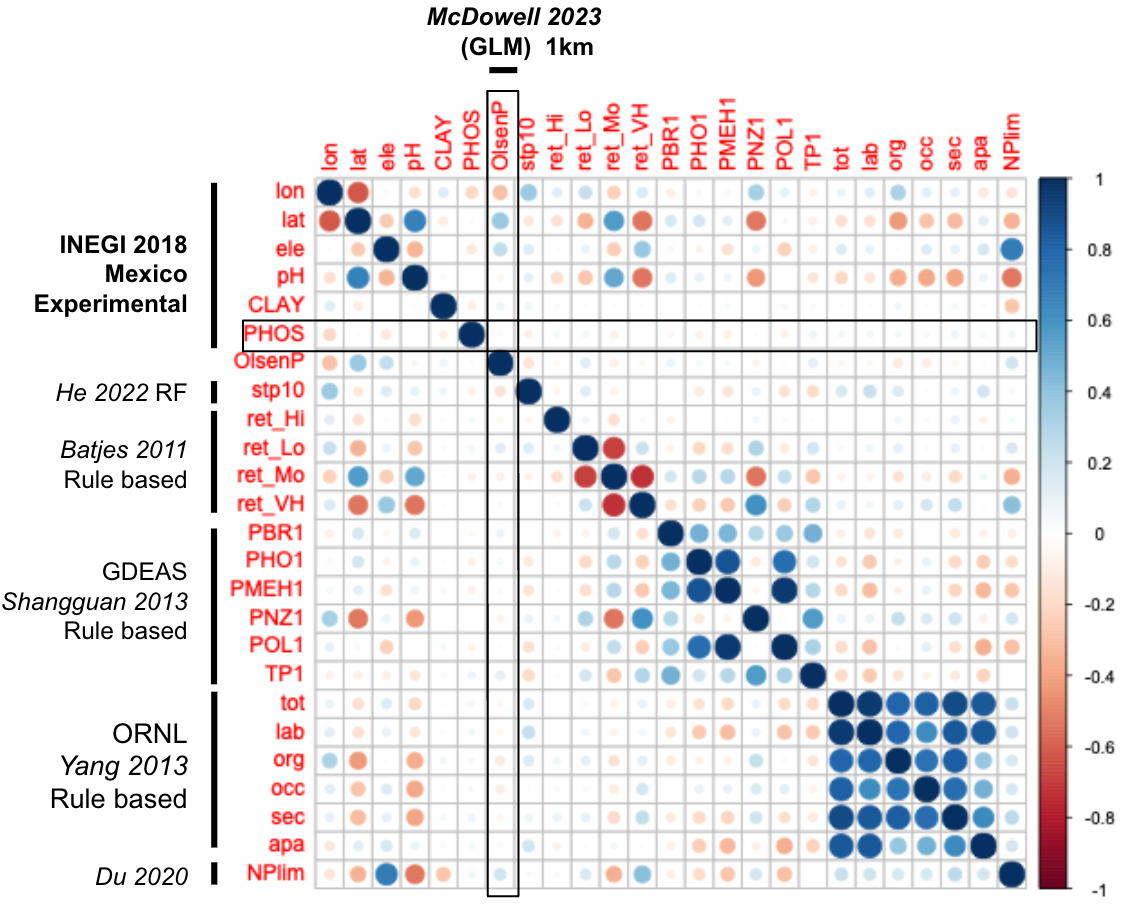
\includegraphics[width=0.65\paperwidth]{Chapter-2/figs/PHOS_correlation.png}
\caption[Pearson correlations (r) between experimental soil available phosphorus in Mexico (PHOS) and predicted phosphorus parameters from global models]{\textit{\textbf{Pearson correlations (r) between experimental soil available phosphorus in Mexico (PHOS) and predicted phosphorus parameters from global models.}} Observed values for lon : longitude, lat: latitude, ele: elevation in \citep{inegi2013}, and clay: clay content, pH, and PHOS: plant available phosphorus in \citep{inegi2013}. Predicted probabilities for Lo: Low, Mo: Moderate, Hi: High, and VH: very high phosphorus retention potential soil classes according to \citep{batjes2011}; predicted
stp10: total phosphorus from \citep{hexianjin2022}, lab: labile and tot: total phosphorus from \citep{yang2013}, phosphorus by Bray, Olsen and Mehlich \citep{mehlich1984} methods and New Zealand phosphorus retention  from \citep{shangguan2014}; and predicted NPlim: Nitrogen Phosphorus limitation from \citep{du2020}. } 
\label{fig::phoscorrelation}
\end{figure}
\clearpage

\begin{figure}[!ht]
\centering
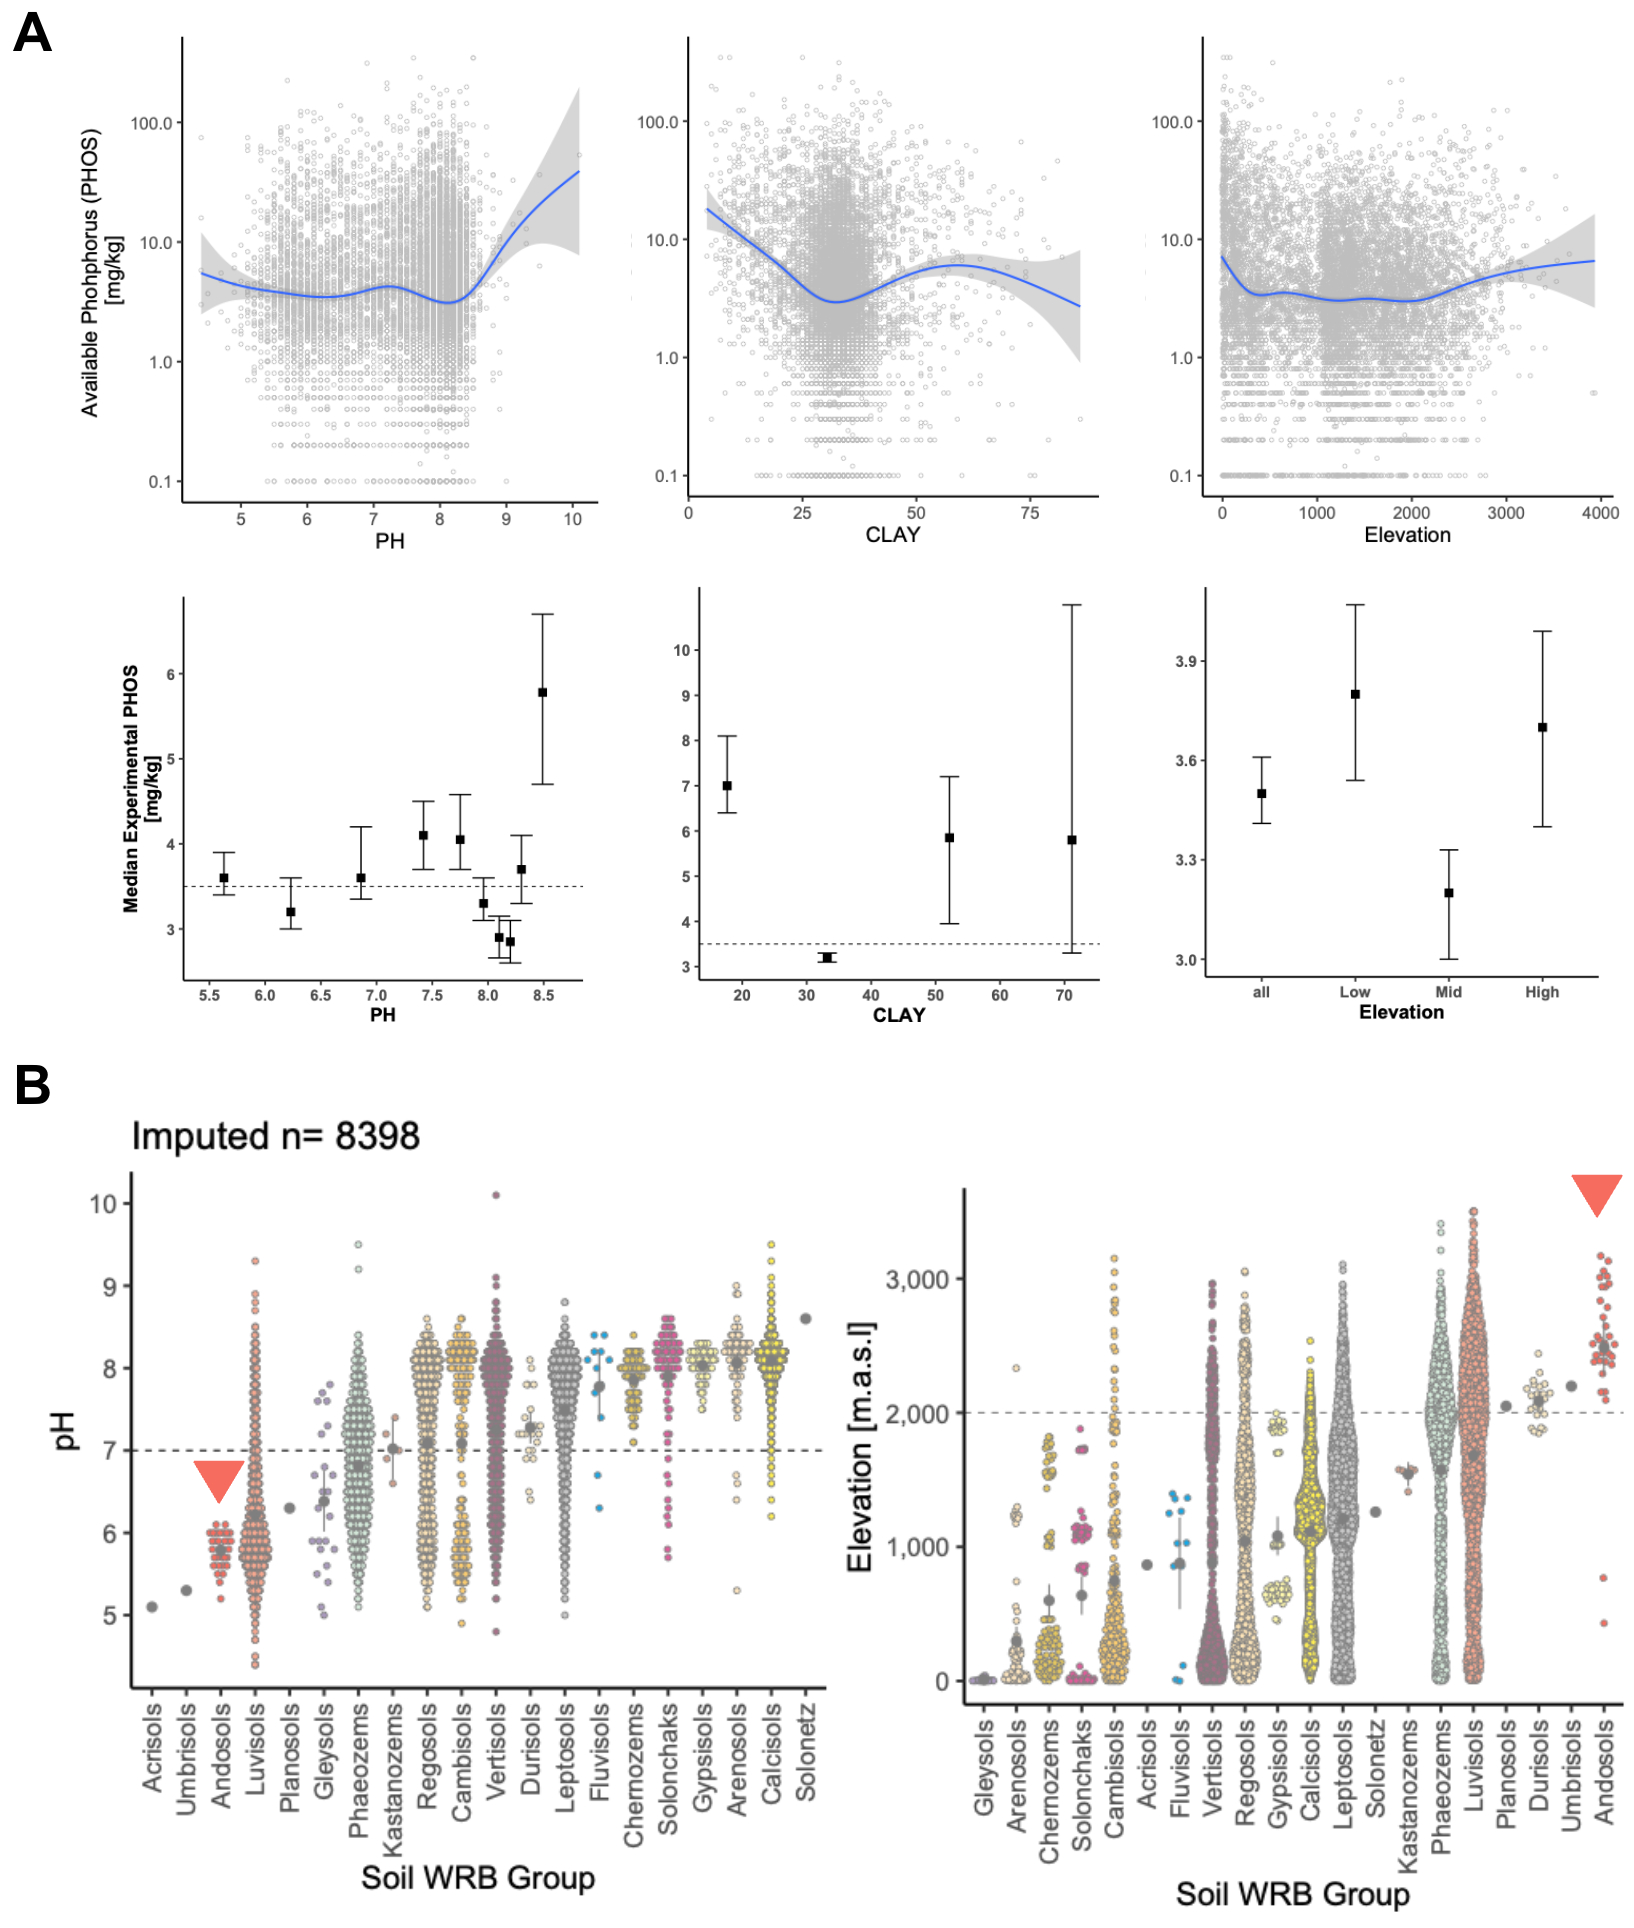
\includegraphics[width=\linewidth]{Chapter-2/figs/marginal_dependencies.png}
\caption[Marginal Dependencies pof PHOS. pH and elevation of WRB soil groups]{\textit{\textbf{Marginal Dependencies pof PHOS, pH and elevation of WRB soil groups.}}}
% \\\hspace{\textwidth} 
\textbf{(A)} 
\textbf{(B)}
\textbf{(C)}
\label{fig::\textbf{(B)}}
\end{figure}
\clearpage



\begin{figure}[!ht]
\centering
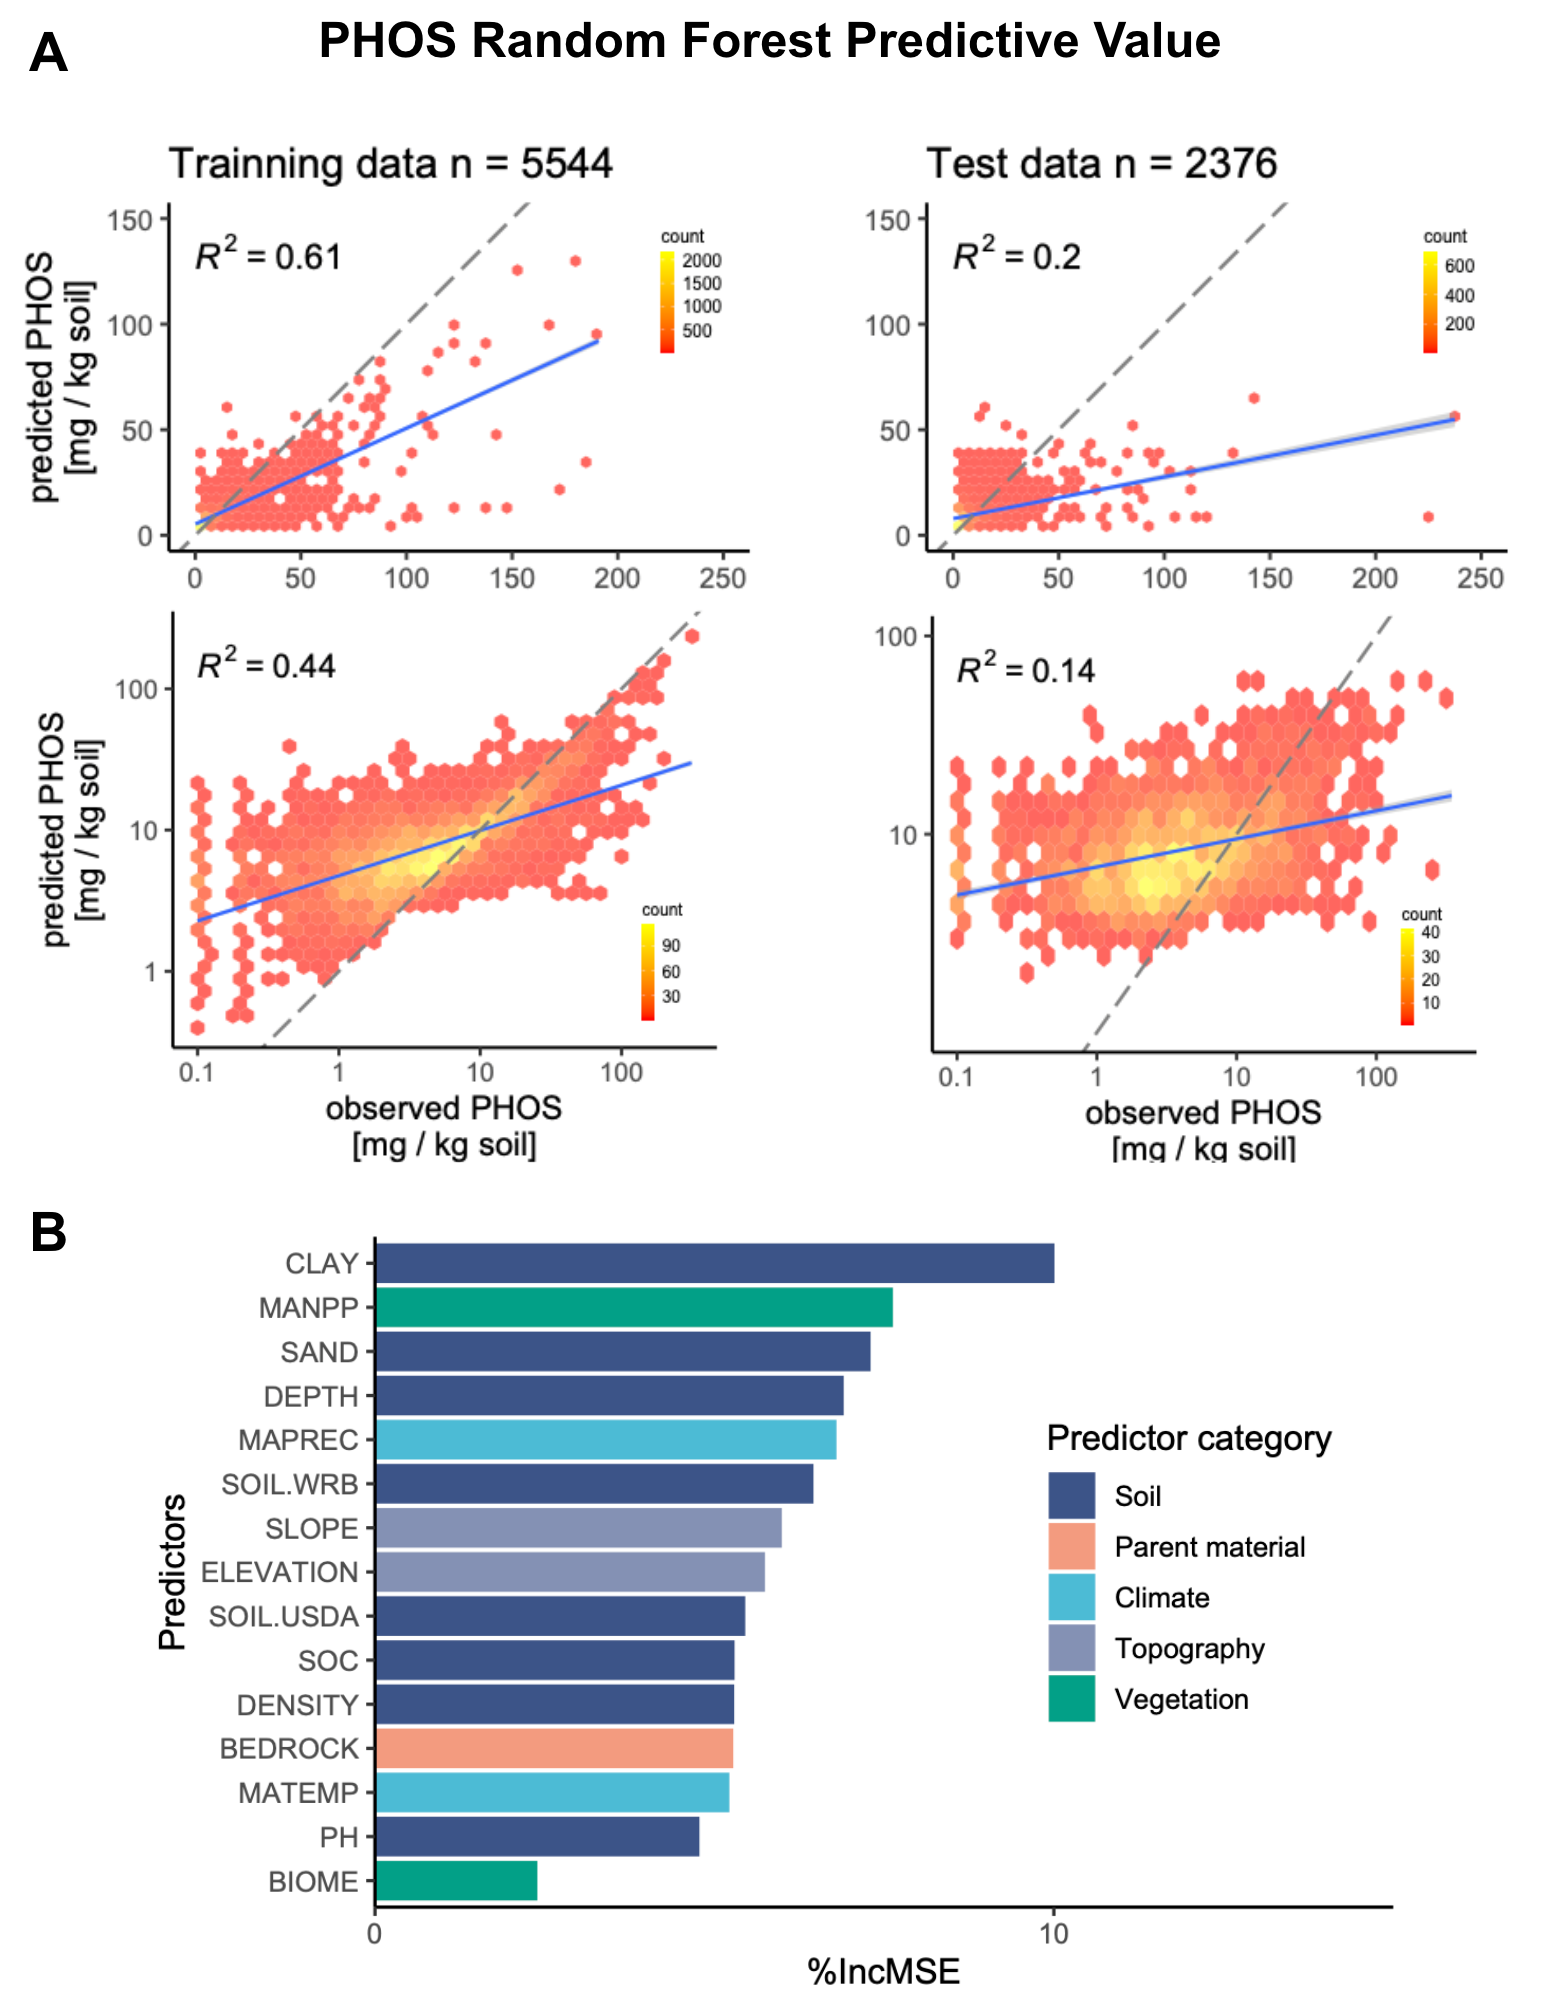
\includegraphics[width=\linewidth]{Chapter-2/figs/rf_validation.png}
\caption[Random forest model validation for soil  available phosphorus PHOS in Mexico]{\textit{\textbf{Random forest model validation for soil  available phosphorus PHOS in Mexico.}} \\\hspace{\textwidth} 
\textbf{(A)} Correlation between observed and predicted available phosphorus in linear (top) and logarithmic (bottom) scales.
The model is over fitted as it has far better predictive value over training $r=0.8$ rather than testing $r=0.4$ data.
\textbf{(B)} Predictor contribution calculated as mean square error difference (\%) after removing it from the model.}
\label{fig::rfvalidation}
\end{figure}
\clearpage



\subsection{Random Forest Model of Olsen and Bray Phosphorus Improves Accuracy of Soil Available Phosphorus Estimation in  Mexico}
After building on the work of \cite{hexianjin2022} and \cite{mcdowell2023}, we increased the predictive value of the soil mapping models for Olsen and Bray extractable phosphorus in the Southern hemisphere. I decided to follow the  Our two hemisphere model increased the Pearson correlation $r$ from 0.0 to 0.7 (0 and 0.5 $R^2$) for observed and predicted values of Olsen P, and  from 0.0 to 0.84 (0 to 0.7 $R^2$) for observed and predicted values of Bray P (Observed-Predicted correlations table 1) in the Southern data.  [Compare mean squared root error]. In addition to this we see good overlap with the training data set for both Africa and LAC (Figure 1C) (MANOVA test), which allows us to make reasonable interpolations. A similar approach increased the total phosphorus predictive value as well from 0.81 to 0.91 (0.65 and 0.81 $R^2$), marginally improving previously reported data for Africa \citep{hengl2017a}, where we expect even less over-fit because of the better sampling and increased mixing of data points in the predictor space.


Appart from the predictive value,  the relative importance of predictors in our models is congruent with the chemical understanding of how phosphorus goes into soil solution.
Phosphorus in solution depends on pH and soil mineralogy, while the total amount of phosphorus in non fertilized soils should depend mostly on parent material and organic mater fractions.
Thus the random forest predictor importance as measured by \%IncMSE in our small model is easier to understand than models including multiple multispectral vegetation indices and climate variables \citep{mcdowell2023}.

This lead us to conclude that we have a more parsimonious model that has better prediction value and better interpretability.

Not only our model shows acceptable and improved internal consistency, but it has increased correlations with other reported measurements of available P. For example for the LAC pixels corresponding to the Hou sampling of Hedley available phosphorus the correlation between our Olsen is 0.5  and Bray is 0.4. For the Africa isDASOIL \citep{miller2021b} extractable phosphorus is 0.4.
At the level of continental and global models our Bray and Olsen predictions have high correlation with McDowell Olsen at the global scale but not in the southern hemisphere, with the predicted water soluble phosphorus in Africa \citep{miller2021b,hengl2017a}and low correlations with previous raster values based on heuristics models like \cite{shangguan2014}, \cite{yang2013} and\cite{batjes2011} retention probabilities (Table1 other prediction correlations).

Although not comparable with prediction values for mean annual temperature,$R^2$ = 0.98 \citep{fick2017}), our model improves prediction for Latin America \cite{mcdowell2023} and a previous model of Africa \citep{hengl2017a} of plant available phosphorus.
Now with the best estimators we had of plant available phosphorus for plants in acicidic and basic soils we proceeded to look for Genome Environment Associations in two crops: Maize heirloom varieties in Mesoamerica and And Sorghum heirlooms in Africa.

\begin{figure}[!ht]
\centering
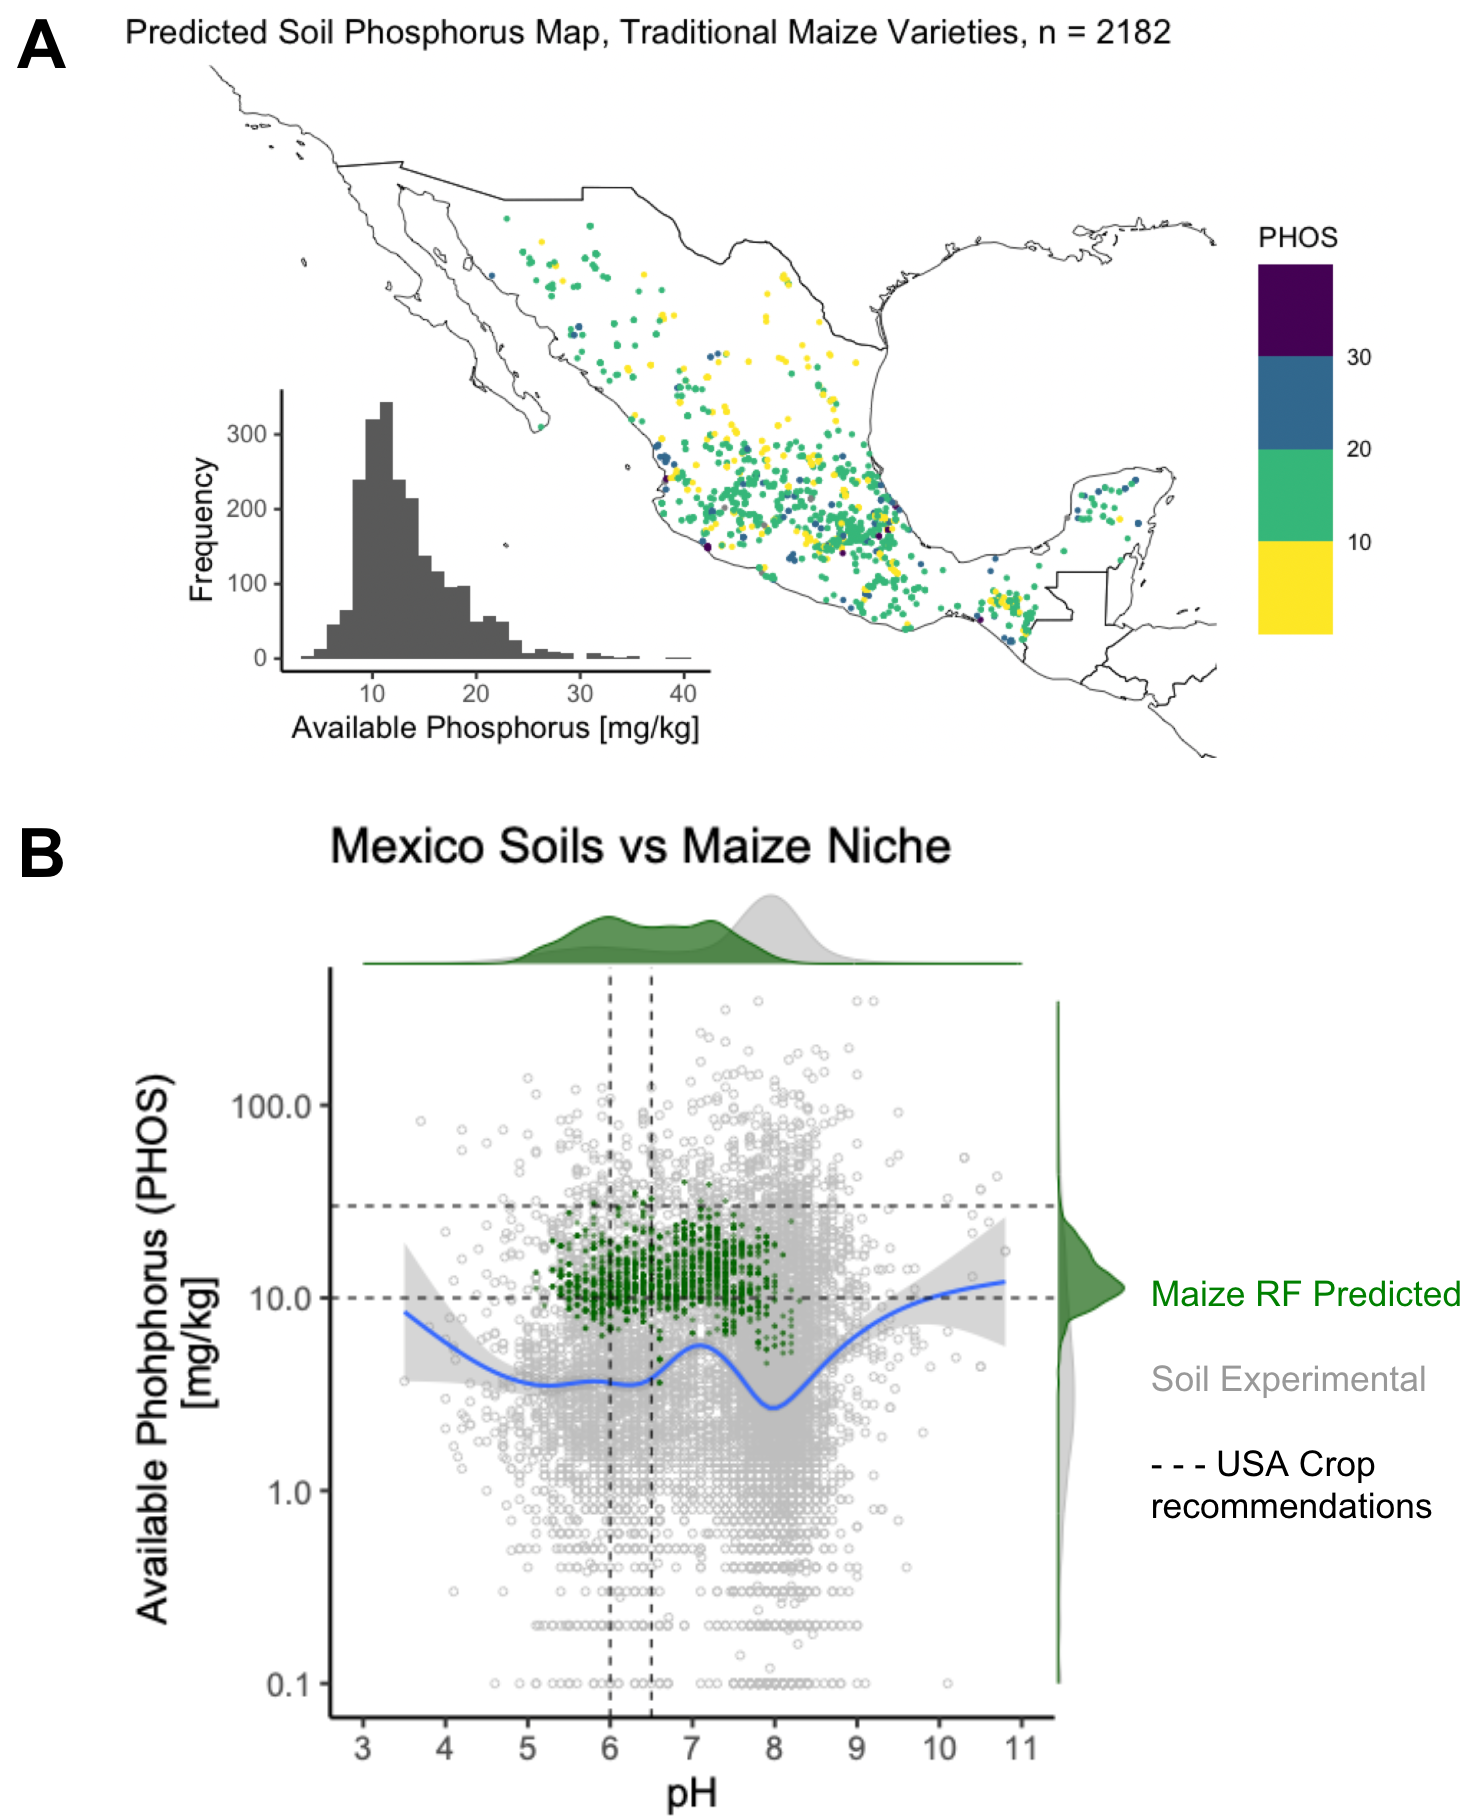
\includegraphics[width=\linewidth]{Chapter-2/figs/predicted_PHOS.png}
\caption[Predicted Available Phosphorus for Mexican Traditional Maize Varieties]{\textit{\textbf{Predicted Available Phosphorus for Mexican Traditional Maize Varieties.}}
\\\hspace{\textwidth}
\textbf{(A)} Geographical distribution for 2350 traditional varieties from the FOAM panel \citep{romero_navarro2017-cn}
\textbf{(B)} Comparison of topsoil phosphorus in 12300 soil samples \citep{paz-pellat2018} with the predictions for the FOAM panel}
\label{fig::pointpred}
\end{figure}
\clearpage

\subsection{Genome Environment Associations Point to Candidate Genes for Adaptation to Divesre Soil Phosphorus Availability Conditions}

\begin{figure}[b]
\centering
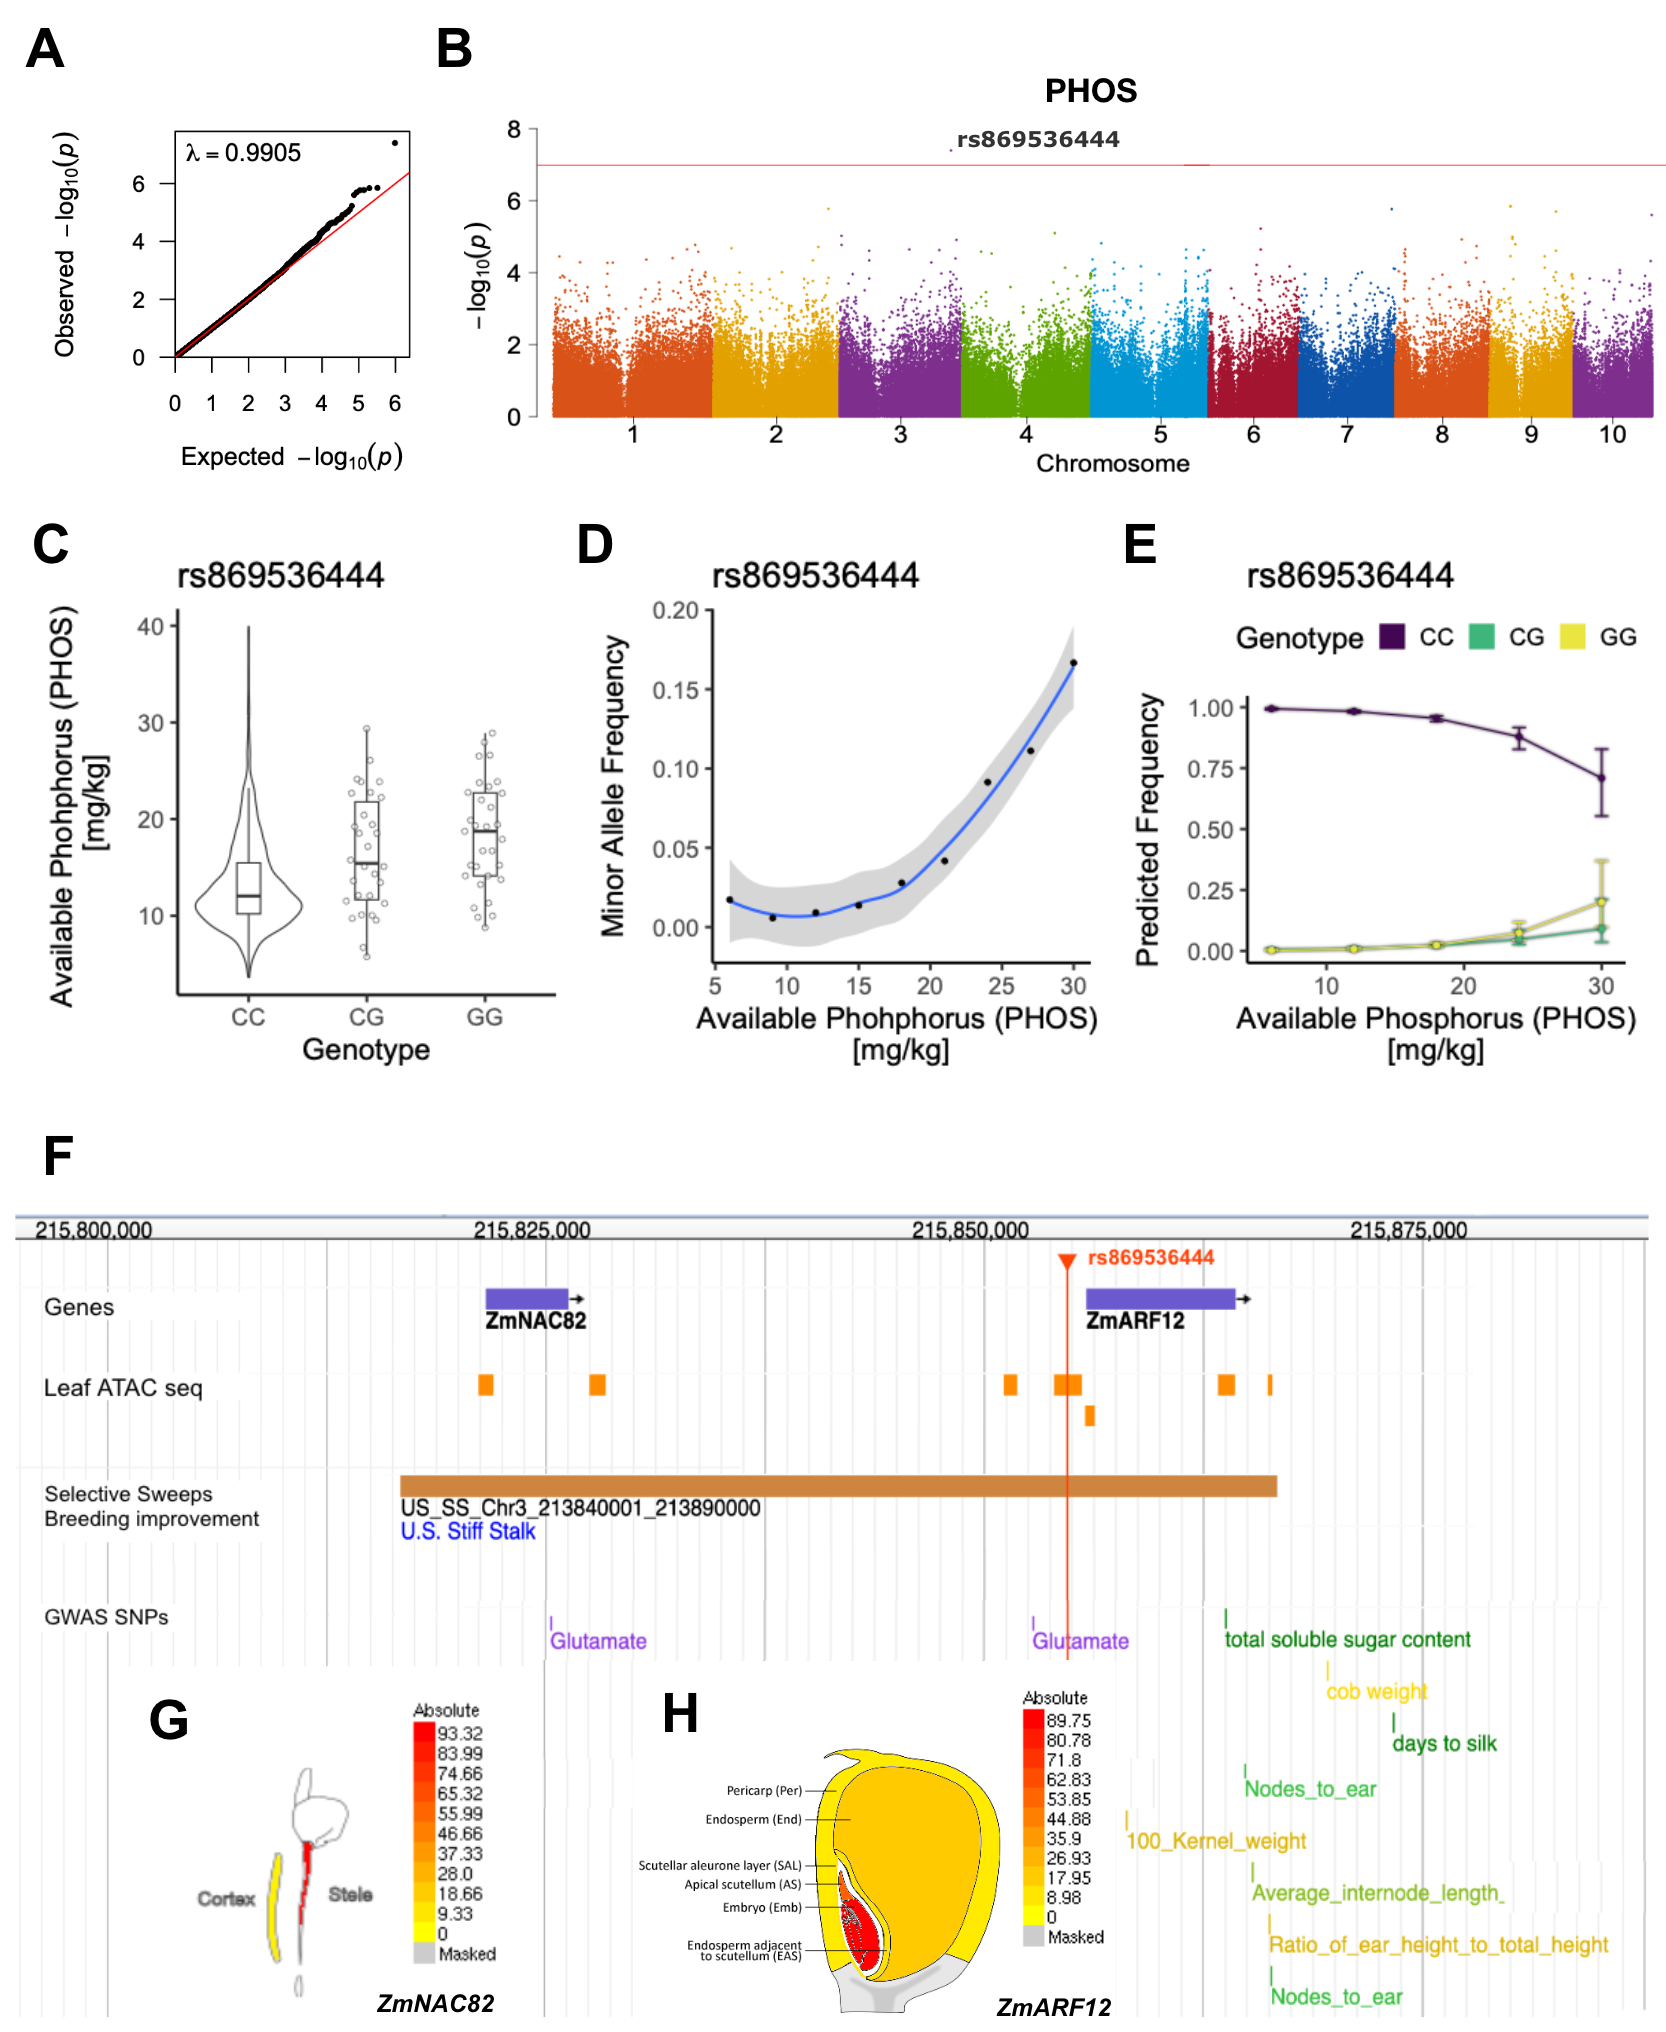
\includegraphics[width=\linewidth]{Chapter-2/figs/PHOS_mlm.png}
\caption[]{}
\label{fig:PHOS_mlm}
\end{figure}
\clearpage

\addtocounter{figure}{-1}
\begin{figure} [t!]
\caption[Linear Mixed Model Association between Maize Genetic Variants and Soil Available Phosphorus in Mexican Traditional Varieties]{\textit{\textbf{Linear Mixed Model Association between Maize Genetic Variants and Soil Available Phosphorus in Mexican Traditional Varieties.}}
\\\hspace{\textwidth}
\textbf{(A)}  \textbf{(B)}  \textbf{(C)} \textbf{(D)} \textbf{(E)}\textbf{(F)} \textbf{(G)} \textbf{(H)} 
 }
\end{figure}

\begin{figure}[!ht]
\centering
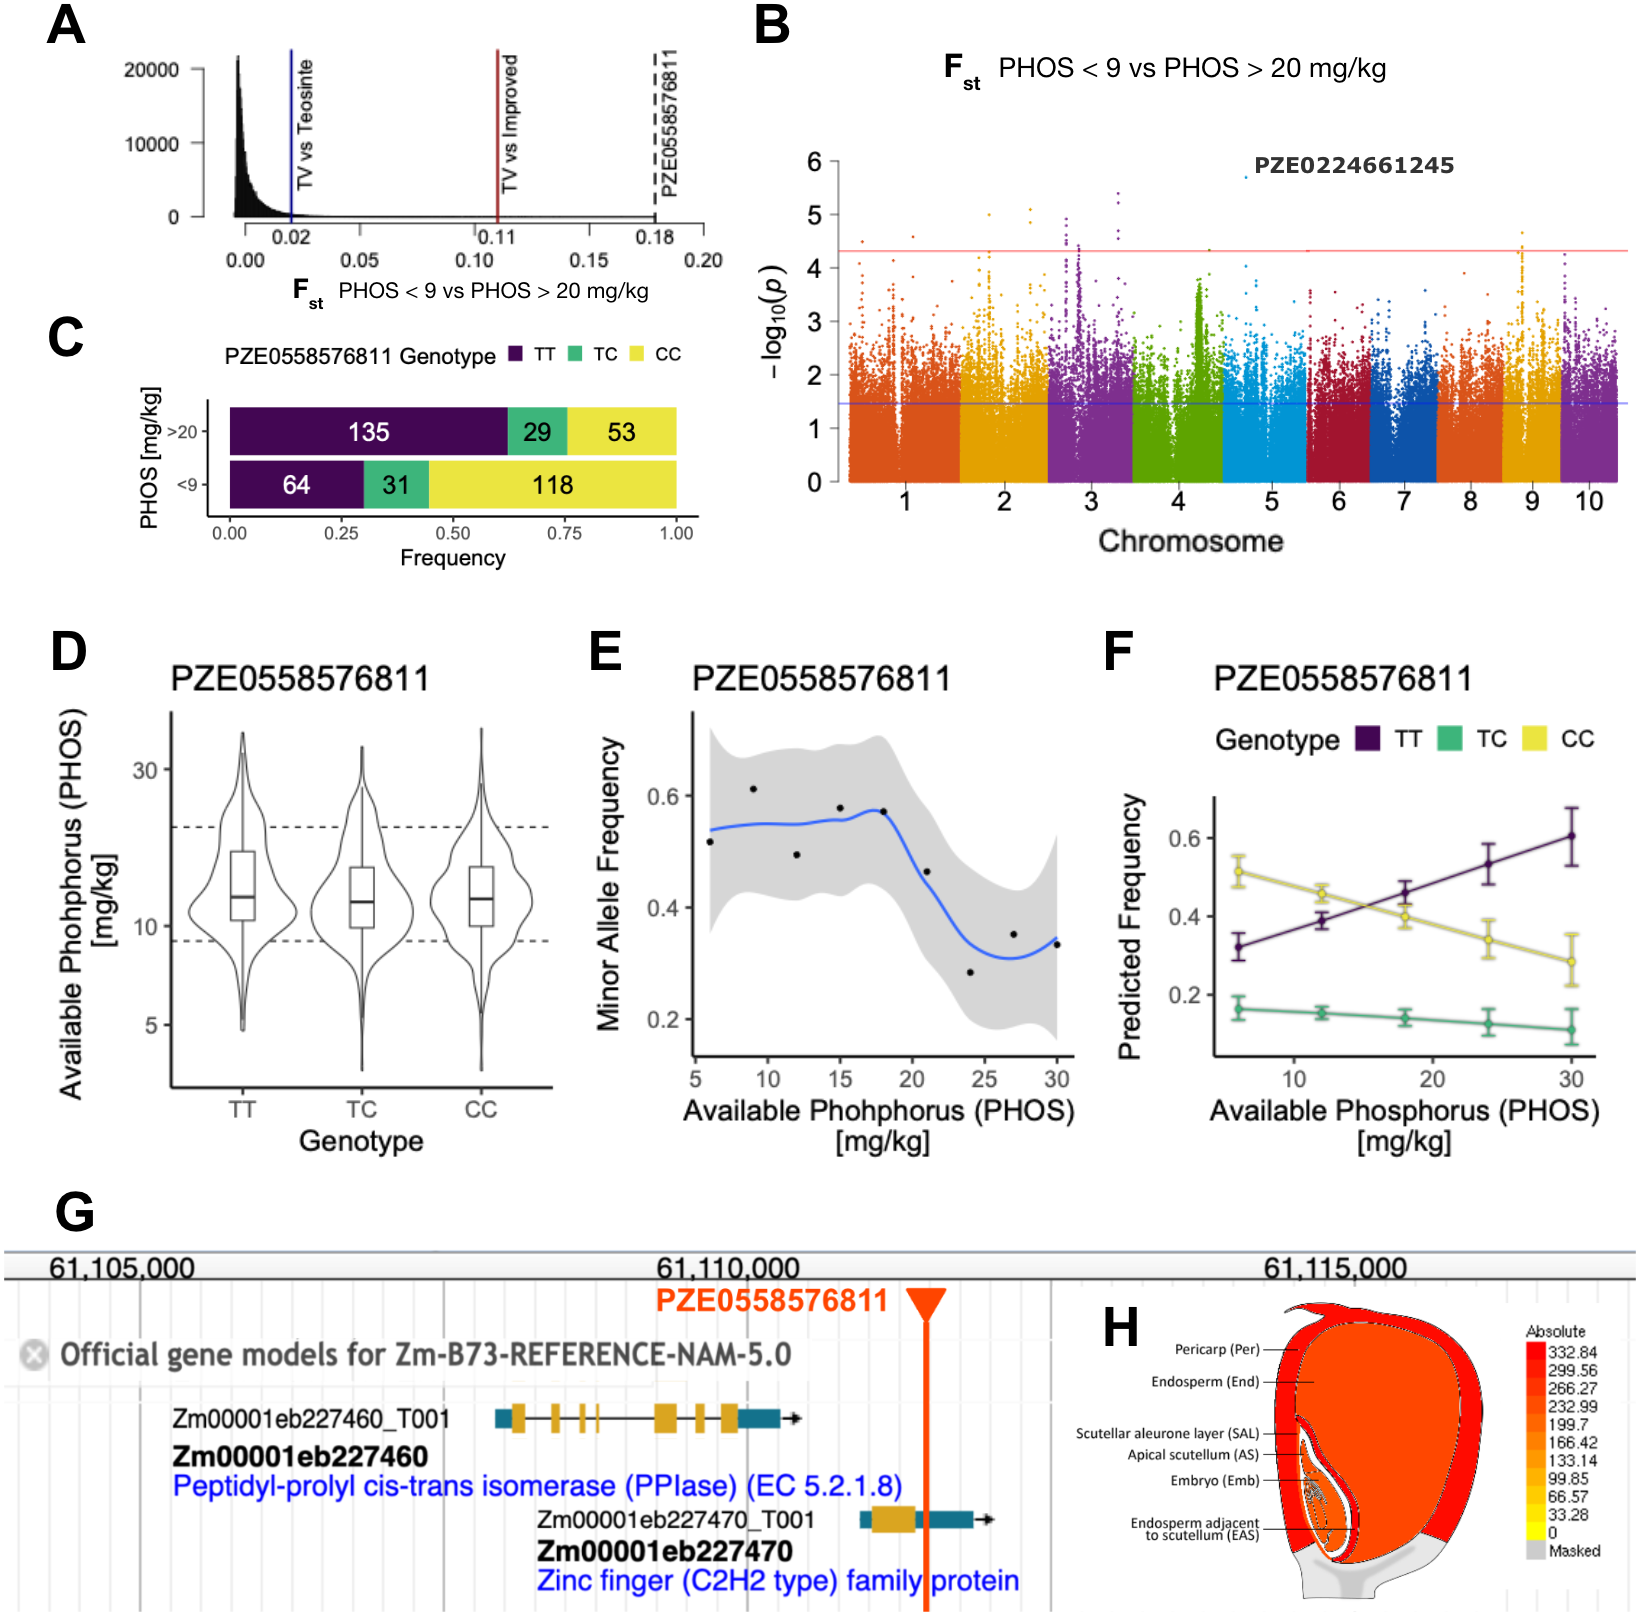
\includegraphics[width=\linewidth]{Chapter-2/figs/PHOS_Fst.png}
\caption[Fst based Association between Maize Genetic Variants and Soil Available Phosphorus in Mexican Traditional Varieties]{\textit{\textbf{ $\boldmath{F_{st}}$ based Association between Maize Genetic Variants and Soil Available Phosphorus in Mexican Traditional Varieties.}}
\\\hspace{\textwidth} 
\textbf{(A)}  \textbf{(B)}  \textbf{(C)} \textbf{(D)} \textbf{(E)}\textbf{(F)} \textbf{(G)} \textbf{(H)} 
 }
\label{fig::PHOS_Fst}
\end{figure}
\clearpage


\printbibliography[heading=subbibintoc, title=References]